% Task 4 – Triển khai Sprint 1
% Nguồn: README.md, CONTRIBUTING.md, docs/process/*.md, apps/*, .github/workflows/ci.yml
\section{Task 4 -- Triển khai Sprint 1}\label{sec:sprint1}

\textbf{Sprint Goal:} có repository, tài liệu có kiểm soát phiên bản, CI tự động trên pull request và MVP xem menu
chạy được (API, màn hình, dữ liệu seed). Sprint kéo dài 2 tuần (02/11 -- 15/11/2026), gồm 9 mục backlog PB-01
$\rightarrow$ PB-09 (22 điểm). Chi tiết: \code{docs/process/sprint-1.md}.

%%%%%%%%%%%%%%%%%%%%%%%%%%%%%%%%%%%%%%%%%%%%%%%%%%%%%%%%%%%%%%%%%%%%%%
\subsection{Task 4.1 -- Thiết lập repository}

Repository GitHub \url{https://github.com/dangpham-work/CupPulse} tổ chức theo monorepo pnpm (ADR-001):

\begin{lstlisting}[basicstyle=\ttfamily\footnotesize,frame=single]
apps/web/            Next.js 15 mobile-first/PWA
apps/api/            NestJS 11: src/modules/<domain>, prisma/, test/
packages/shared/     Kieu du lieu va ham dung chung web <-> API
docs/                requirements/, diagrams/, architecture/, process/
tests/               Integration/E2E xuyen ung dung (Sprint 2)
.github/workflows/   ci.yml
docker-compose.yml   .env.example   README.md   CONTRIBUTING.md
\end{lstlisting}

\begin{longtable}{|p{4.2cm}|p{10.6cm}|}
\caption{Yêu cầu Task 4.1 và hiện thực}\label{tab:t41}\\
\hline
\thead \textbf{Yêu cầu} & \textbf{Hiện thực} \\ \hline
\endfirsthead
\hline
\thead \textbf{Yêu cầu} & \textbf{Hiện thực} \\ \hline
\endhead
Cấu trúc \code{apps/web}, \code{apps/api}, \code{docs} & Monorepo pnpm workspace; thêm \code{packages/shared} cho kiểu dữ liệu dùng chung \\ \hline
Chiến lược branch, pull request & GitHub Flow: \code{main} được bảo vệ, nhánh \code{feat/}, \code{fix/}, \code{docs/}, \code{ci/}; mọi thay đổi qua PR có template (mục đích, \textbf{lý do}, mã yêu cầu, cách kiểm tra) \\ \hline
\code{README.md}, \code{.gitignore}, \code{.env.example} & README hướng dẫn chạy local (Docker Compose hoặc pnpm), test, build; \code{.env.example} liệt kê đủ biến, không chứa secret thật \\ \hline
Issue board / Product Backlog & 26 issue PB-01 $\rightarrow$ PB-26 trên GitHub Issues, milestone \texttt{Sprint 1}, \texttt{Sprint 2}, nhãn \texttt{type:*}, \texttt{priority:*}, \texttt{area:*}; bản gốc \code{docs/process/product-backlog.md} \\ \hline
Quy ước commit, Definition of Done & Conventional Commits (\code{feat(api): ...}); DoD 8 tiêu chí trong \code{CONTRIBUTING.md} \\ \hline
\end{longtable}

\textbf{Definition of Done} (tóm tắt): đạt tiêu chí chấp nhận trong SRS; có test tự động; lint, typecheck, test, build
pass và CI xanh; validate đầu vào ở backend; dùng tốt ở 360 px; không lộ secret; cập nhật ma trận truy vết và tài
liệu; merge qua PR.

%%%%%%%%%%%%%%%%%%%%%%%%%%%%%%%%%%%%%%%%%%%%%%%%%%%%%%%%%%%%%%%%%%%%%%
\subsection{Task 4.2 -- Quản lý tài liệu}

Toàn bộ tạo phẩm Task 1--3 nằm trong \code{docs/}, có mục lục và bảng lịch sử thay đổi ở \code{docs/README.md}.
Mỗi task vào \code{main} bằng một pull request riêng, mô tả rõ lý do:

\begin{table}[H]
\centering
\caption{Lịch sử thay đổi tài liệu qua pull request}\label{tab:doc-history}
\begin{tabularx}{\textwidth}{|c|l|X|}
\hline
\thead \textbf{PR} & \textbf{Nhánh} & \textbf{Nội dung và lý do} \\ \hline
\#1 & \code{docs/task1-requirements} & Task 1: bối cảnh, SRS, use-case -- khởi tạo yêu cầu \\ \hline
\#2 & \code{docs/task2-modeling} & Task 2: activity, sequence, class, state diagram -- mô hình hóa từ SRS \\ \hline
\#3 & \code{docs/task3-architecture} & Task 3: C4, 9 ADR, deployment diagram -- thiết kế trước khi hiện thực \\ \hline
\#30 & \code{feat/task4-sprint1} & Task 4: mã nguồn Sprint 1, CI, quy trình; ma trận truy vết v0.4 -- hiện thực FR-01, FR-02 (API) \\ \hline
\end{tabularx}
\end{table}

Thay đổi quyết định kiến trúc được ghi bằng ADR mới; ADR cũ chỉ đổi trạng thái \textit{Superseded}.

%%%%%%%%%%%%%%%%%%%%%%%%%%%%%%%%%%%%%%%%%%%%%%%%%%%%%%%%%%%%%%%%%%%%%%
\subsection{Task 4.3 -- MVP Sprint 1}

\begin{longtable}{|p{3.6cm}|p{6.6cm}|p{4.6cm}|}
\caption{Phạm vi MVP Sprint 1}\label{tab:mvp1}\\
\hline
\thead \textbf{Hạng mục} & \textbf{Hiện thực} & \textbf{Mã nguồn} \\ \hline
\endfirsthead
\hline
\thead \textbf{Hạng mục} & \textbf{Hiện thực} & \textbf{Mã nguồn} \\ \hline
\endhead
\code{GET /products} & Món \code{isActive = true}; \code{inStock = stock > 0}; lọc \code{?category=}; không cần token & \code{apps/api/src/modules/ catalog/} \\ \hline
\code{GET /products/:id} & Kèm \code{sizes}, \code{toppings}; 404 \code{PRODUCT\_NOT\_FOUND}; 400 khi id không phải UUID & \code{catalog.controller.ts}, \code{catalog.service.ts} \\ \hline
Lỗi và validate & Định dạng \code{\{statusCode, code, message\}}; query lạ bị từ chối (whitelist); lỗi hệ thống không lộ chi tiết & \code{common/}, \code{app.setup.ts} \\ \hline
Màn menu mobile-first & Lưới 2 cột ở 360 px, tab danh mục, nhãn ``Hết hàng'', vùng chạm $\ge$ 44 px & \code{apps/web/src/features/ menu/} \\ \hline
Loading / empty / error & Skeleton; ``Chưa có món nào''; thông báo lỗi + nút ``Thử lại'' gọi lại API & \code{MenuView.tsx} \\ \hline
Dữ liệu mẫu & Migration Prisma (kèm CHECK giá, tồn kho $\ge$ 0) và seed idempotent: 4 danh mục, 13 sản phẩm (1 hết hàng, 1 đã ẩn), 4 topping & \code{apps/api/prisma/} \\ \hline
Health check & \code{GET /health} ping DB, trả 200 hoặc 503 & \code{modules/health/} \\ \hline
Chạy local & \code{docker compose up --build}: web, API (tự migrate + seed), PostgreSQL & \code{docker-compose.yml}, \code{apps/*/Dockerfile} \\ \hline
\end{longtable}

\begin{figure}[H]
\centering
\begin{minipage}{0.27\textwidth}\centering
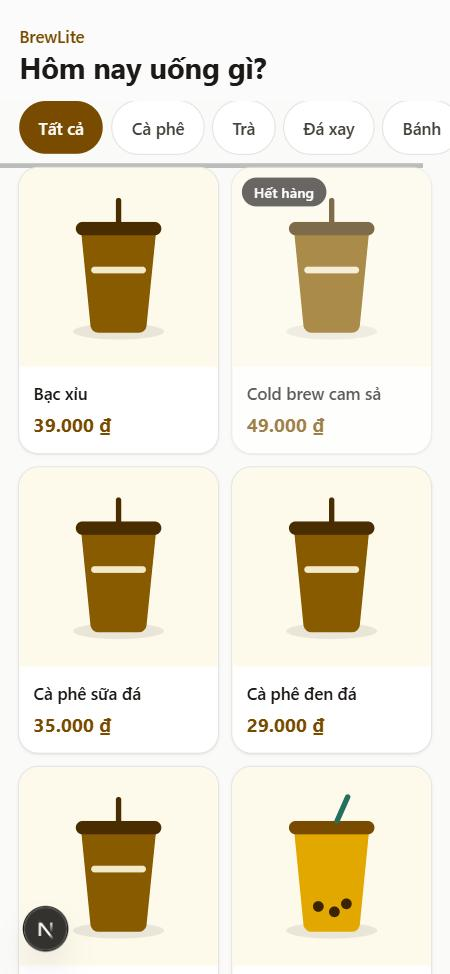
\includegraphics[width=\linewidth]{figures/menu-mobile.jpg}
\end{minipage}\hspace{1cm}
\begin{minipage}{0.27\textwidth}\centering
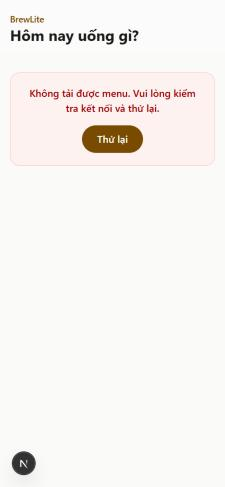
\includegraphics[width=\linewidth]{figures/menu-error.jpg}
\end{minipage}
\caption{Màn menu ở chiều rộng mobile: dữ liệu từ API (trái) và trạng thái lỗi khi API không phản hồi (phải)}\label{fig:menu}
\end{figure}

\newpage
\subsubsection*{Kiểm thử Sprint 1}

\begin{longtable}{|p{2.0cm}|p{3.4cm}|p{6.0cm}|c|}
\caption{Test tự động Sprint 1}\label{tab:tests1}\\
\hline
\thead \textbf{Mã} & \textbf{Loại} & \textbf{Nội dung} & \textbf{Số ca} \\ \hline
\endfirsthead
\hline
\thead \textbf{Mã} & \textbf{Loại} & \textbf{Nội dung} & \textbf{Số ca} \\ \hline
\endhead
UNIT-T07, T08 & Unit (Jest) & \code{CatalogService}: lọc, ánh xạ \code{inStock}, topping ngừng bán, \code{PRODUCT\_NOT\_FOUND}; kiểm tra biến môi trường & 8 \\ \hline
API-T01, T02 & API (Jest + supertest, Prisma giả lập) & 200 không token, lọc danh mục, query lạ $\rightarrow$ 400, id sai $\rightarrow$ 400, 404, lỗi DB $\rightarrow$ 500, \code{/health} 200/503 & 9 \\ \hline
INT-T08 & Integration (PostgreSQL thật) & Migrate + seed từ DB trống; 12 món đang bán, size, topping, món ẩn $\rightarrow$ 404 & 5 \\ \hline
UI-T01 & Component (Vitest + Testing Library) & Skeleton, danh sách, empty, lỗi + Thử lại, mất mạng, ``Hết hàng'', tab danh mục & 7 \\ \hline
UNIT-T09 & Unit (node:test) & \code{formatVnd} theo quy ước \texttt{45.000 ₫} & 2 \\ \hline
\multicolumn{3}{|r|}{\textbf{Tổng}} & \textbf{31} \\ \hline
\end{longtable}

Test được viết trước phần hiện thực. Để chắc test thật sự kiểm tra hành vi, nhóm cố ý làm sai logic (đổi
\code{stock > 0} thành \code{stock >= 0}, đổi nhãn ``Hết hàng'') và xác nhận test tương ứng chuyển sang thất bại.

%%%%%%%%%%%%%%%%%%%%%%%%%%%%%%%%%%%%%%%%%%%%%%%%%%%%%%%%%%%%%%%%%%%%%%
\subsection{Task 4.4 -- Continuous Integration}

Workflow \code{.github/workflows/ci.yml} chạy khi mở hoặc cập nhật pull request vào \code{main} và khi push lên
\code{main}:

\begin{center}
\begin{tikzpicture}[
  st/.style={draw=brew, fill=brewlight, rounded corners=3pt, minimum height=0.8cm, align=center, font=\scriptsize\bfseries},
  arr/.style={-latex, thick}]
  \node[st] (a) {Install};
  \node[st, right=0.3cm of a] (b) {Lint};
  \node[st, right=0.3cm of b] (c) {Typecheck};
  \node[st, right=0.3cm of c] (d) {Unit Test};
  \node[st, right=0.3cm of d] (e) {Build};
  \node[st, below=0.5cm of b] (f) {Integration Test\\(PostgreSQL service)};
  \node[st, below=0.5cm of d] (g) {Docker build\\(web, api)};
  \draw[arr] (a) -- (b); \draw[arr] (b) -- (c); \draw[arr] (c) -- (d); \draw[arr] (d) -- (e);
\end{tikzpicture}
\end{center}

Job \textit{quality} chạy tuần tự Install $\rightarrow$ Lint $\rightarrow$ Typecheck $\rightarrow$ Unit Test
$\rightarrow$ Build; job \textit{integration} dựng PostgreSQL 16 làm service container, chạy migrate, seed hai lần
(kiểm tra seed idempotent) rồi integration test; job \textit{docker} build image web và API để kiểm tra Dockerfile.
\textbf{Branch protection} của \code{main} yêu cầu cả ba job pass
mới được merge (NFR-16).

% Minh chứng CI – nguồn: docs/process/sprint-1.md mục 4
\subsubsection*{Minh chứng pipeline}

\begin{longtable}{|p{3.0cm}|p{1.5cm}|p{6.3cm}|p{3.8cm}|}
\caption{Các lần chạy CI của Sprint 1}\label{tab:ci-runs}\\
\hline
\thead \textbf{Lần chạy} & \textbf{Commit} & \textbf{Kết quả} & \textbf{Link} \\ \hline
\endfirsthead
\hline
\thead \textbf{Lần chạy} & \textbf{Commit} & \textbf{Kết quả} & \textbf{Link} \\ \hline
\endhead
PR \#30 -- lần 1 & \code{96a0197} & \textbf{Cancelled}: commit mới được push nên workflow tự hủy lượt cũ & \href{https://github.com/dangpham-work/CupPulse/actions/runs/41408066493}{run 41408066493} \\ \hline
PR \#30 -- lần 2 & \code{cd3f53d} & \textbf{Success}: quality 1m 0s, integration 43s, docker 1m 53s & \href{https://github.com/dangpham-work/CupPulse/actions/runs/41408203576}{run 41408203576}, \href{https://github.com/dangpham-work/CupPulse/pull/30}{PR \#30} \\ \hline
PR \#31 (minh chứng lỗi) & \code{89d5753} & \textbf{Failure} ở bước \textbf{Lint}: biến không dùng; Typecheck, Unit Test, Build bị bỏ qua; job Docker cũng đỏ vì \code{next build} chạy ESLint & \href{https://github.com/dangpham-work/CupPulse/actions/runs/41408237890}{run 41408237890}, \href{https://github.com/dangpham-work/CupPulse/pull/31}{PR \#31} (đóng, không merge) \\ \hline
\end{longtable}

\begin{figure}[H]
\centering
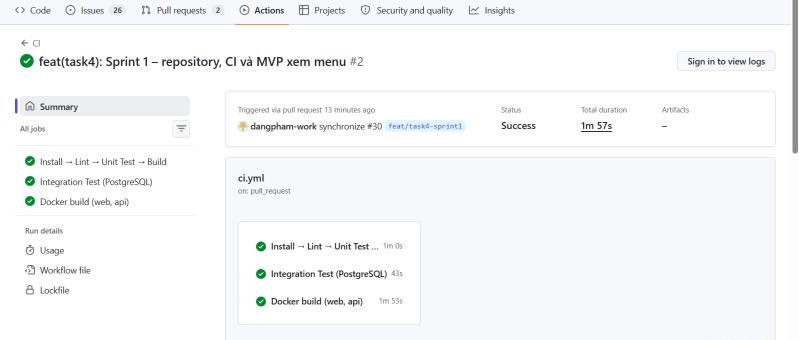
\includegraphics[width=0.9\textwidth]{figures/ci-pass.png}
\caption{CI của PR \#30 thành công: ba job xanh}\label{fig:ci-pass}
\end{figure}

\begin{figure}[H]
\centering
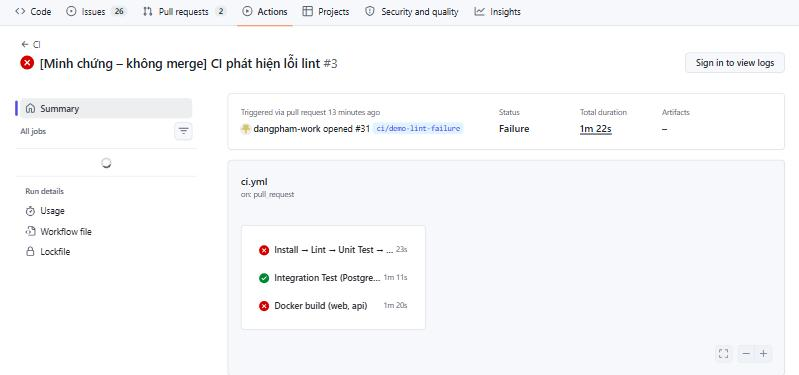
\includegraphics[width=0.9\textwidth]{figures/ci-fail.png}
\caption{CI của PR \#31 phát hiện lỗi lint: job chất lượng và job Docker đỏ}\label{fig:ci-fail}
\end{figure}

Trích log bước Lint của run 41408237890:

\begin{lstlisting}[basicstyle=\ttfamily\scriptsize,frame=single]
apps/web lint:   27:7  error  'unusedForCiDemo' is assigned a value but never used
                 @typescript-eslint/no-unused-vars
apps/web lint: x 1 problem (1 error, 0 warnings)
\end{lstlisting}

\textbf{Sự cố trong Sprint.} Mẫu \code{.gitignore} Python có dòng \code{lib/} làm
\code{apps/web/src/lib/api.ts} không được commit ở lần push đầu (máy local vẫn build được vì tệp có trên đĩa). Lỗi
được phát hiện khi chuẩn bị nhánh minh chứng, trước khi lượt CI đầu chạy xong, và được sửa ở commit \code{cd3f53d}.
Bài học: CI trên máy sạch là nơi kiểm chứng repository đầy đủ, nên luôn chờ CI xanh trước khi merge.

